\documentclass{article}
\usepackage{xyreport}

\makeatletter
\def\maketitle{%
%  \vfill
  \begin{center}%\leavevmode
    \vspace{1em}
    \normalfont
    {\sanhao \bf \@title\par}%
    \vspace{2em}   %缩小题目和作者名字之间的行距,这里是1毫米
    {\xiaosi \@author\par}%
    \vspace{2em}
    {\xiaosi \@date\par}%去掉%显示日期
    \vspace{4em}
  \end{center}%
%  \vfill
  }
\makeatother
\graphicspath{{figures/}}
\title{网格简化实验报告}
\date{\today}
\author{基科11 刘心宇 2011012135}
\begin{document}
\maketitle
\tableofcontents
\newpage
\section{实验目的}
实现基于二次误差度量的网格简化算法。\cite{garland1997surface}
\section{实验内容}
导入三角网格模型(obj文件),按一定比例进行简化,并输出。
\section{实验原理}
Hoppe的边收缩(edge collapse)操作\cite{hoppe1993mesh,hoppe1996progressive}可推广为一般的顶点
合并变换来描述$(v_1,v_2)\rightarrow v$,其含义是将场景中的两个
顶点 $(v_1,v_2)$移到一新的位置 $v$,将连向 $(v_1,v_2)$的所有边都
连向$v$,并删除所有退化的边和面片。
\subsection{点对合并}
\label{sec:tiaojian}
其中点对$(v_1,v_2)$合并的原则
\begin{enumerate}
\item $(v_1,v_2)$为某一表面上的相邻点,即$(v_1,v_2)$为一条边,如图~\ref{fig:EC}
\begin{figure}[H]
    \centering
    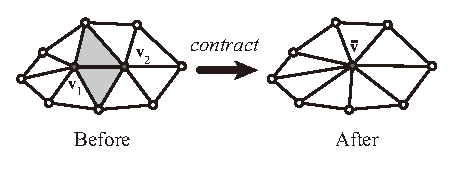
\includegraphics[width=0.6\textwidth]{1.eps}
    \caption{Edge contraction}
    \label{fig:EC}
\end{figure}
\item $||v_1-v_2||<t$,$t$为用户给定的阈值参数,如图~\ref{fig:NEC}
\begin{figure}[H]
    \centering
    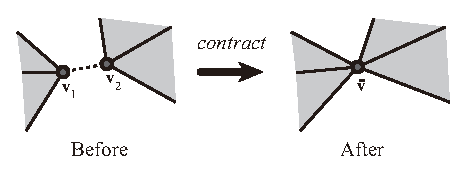
\includegraphics[width=0.6\textwidth]{2.eps}
    \caption{Non-edge contraction}
    \label{fig:NEC}
\end{figure}
\end{enumerate}
\subsection{二次误差度量} 
Garland和Heckbert引进了二次误差度量来刻划每一个顶点移动后引起的误差。对表面上的每一个顶点均有许多三角面片与之相邻,记$plane(v_a)$ 为这些三角形所在的平面方程所构成的集合,即
\begin{equation}
plane(v_a)=\left\{(a,b,c,d)\left|
\begin{array}{c}
ax+by+cz+d=0,(a^2+b^2+c^2=1)\\
\mathrm{is \ coefficients \ of \ the \ adjacent \ plane \ of} \ v_a
\end{array} 
\right\}\right.
\end{equation}
则我们采用如下的二次函数来度量$v_a$移动到$v$时产生的误差
\begin{equation}
\label{equ:wucha}
    \Delta(v_a\rightarrow v)=\sum_{p\in plane(v_a)}(pv^T)^2
\end{equation}
其中$v=(x,y,z,1)$为齐次坐标。展开公式~\eqref{equ:wucha}得到
\begin{equation}
\label{equ:zhankai}
\Delta(v_a\rightarrow v)=\sum_{p\in plane(v_a)}(pv^T)^2=v(\sum_{p\in plane(v_a)}K_p)v^T=vQ(v_a)v^T
\end{equation}
式~\eqref{equ:zhankai}中
\begin{equation}
K_p=p^Tp=\left[ 
\begin{array}{cccc}
a^2 & ab & ac & ad\\
ab & b^2 & bc & bd\\
ac & bc & c^2 & cd\\
ad & bd & cd & d^2
\end{array}
\right]
\end{equation}
这样,对每一顶点 $v_a$,在预处理时,我们均可按上述方法计算矩阵$Q(v_a)$,进而就可对其移动进行误差度量了。但由于每次合并时,需同时移动两点,故必须考虑同时移动多个顶点后形成的误差。
\subsection{多点移动的误差} 
Garland和Heckbert简单地采用加法规则来刻划多点移动而形成的误差,对点对合并$(v_1,v_2)\rightarrow v$,其误差为$\Delta(v)=\Delta(v_1\rightarrow v)+\Delta(v_2\rightarrow v)=v(Q(v_1)+Q(v_2))v^T=vQv^T$,其中。因而,应选取$v$使误差达到最小。\par
由极值的性质知,$v$满足系统方程$$\dfrac{\partial \Delta(v)}{\partial x}=\dfrac{\partial \Delta(y)}{\partial y}=\dfrac{\partial \Delta(z)}{\partial z}=0$$
即
\begin{equation}
\label{equ:zuizhi}
\left[ 
\begin{array}{cccc}
q_{11} & q_{12} & q_{13} & q_{14} \\
q_{12} & q_{22} & q_{23} & q_{24} \\
q_{13} & q_{23} & q_{33} & q_{34} \\
0 & 0 & 0 & 1
\end{array}
\right]v=
\left[ 
\begin{array}{c}
0\\0\\0\\1
\end{array}
\right]
\end{equation}\par
若式~\eqref{equ:zuizhi}有唯一解,则其解为$v$的最优解。否则,用伪逆技术求$v$。若伪逆技术失败,则简单地选取$v$为$(v_1,v_2)$或者$\dfrac{v_1+v_2}{2}$中的任何一个。
\section{编程实现}
\subsection{算法描述}
基于二次误差度量的网格简化算法如下
\begin{enumerate}
\item 计算所有顶点的二次误差度量矩阵$Q$
\item 选择所有符合~\ref{sec:tiaojian}中条件的顶点对$P_{ij}=(v_i,v_j)$。
\item 计算每一个顶点对$P_{ij}$最优的目标顶点$\overline{v_{ij}}$。将误差$C_{ij}=\overline{v_{ij}}^T(Q_i+Q_j)\overline{v_{ij}}$作为收缩该顶点对~$P_{ij}$的代价(cost)
\item 按照顶点对的代价$C_{ij}$,生成最小堆(heap)\cite{leiserson2001introduction}
\item 收缩代价最小的顶点对$P_{ij}$,移除多余的顶点,更新包含$v_i$和$v_j$的顶点对的代价$C_{im},C_{nj}$。反复执行,直到满足简化条件
\end{enumerate}
\subsection{文件结构}
\begin{tabbing}
\hspace*{2em}\=文件\hspace*{8em} \=说明\hspace*{20em}\kill
\>.$\backslash$SimpleObject.h\>定义辅助类,包括误差矩阵QMat,堆Heap等\\
\>.$\backslash$SimpleObject.cpp\>实现网格简化算法的主要代码\\
\>.$\backslash$XYTime.cpp\>计时模块\\
\>.$\backslash$Main.cpp\>测试用例\\\\
\>//网格模型解析(助教提供,有部分改动)\\
\>.$\backslash$SimpleObject.h\>\\
\>.$\backslash$Vec3f.h\>\\
\>.$\backslash$SimpleObject.cpp\>\\
\>.$\backslash$Vec3f.cpp\>
\end{tabbing}
\subsection{使用说明}
\begin{verbatim}
    <inputfile> <option>
    available parameters
    -r <rate> : Set the coefficient of simplification
    -h        : Show help
\end{verbatim}
\section{效果演示}
\begin{figure}[H]
  \centering%
  \subfloat[$\times$1.0 \ 46398 \ faces]{
    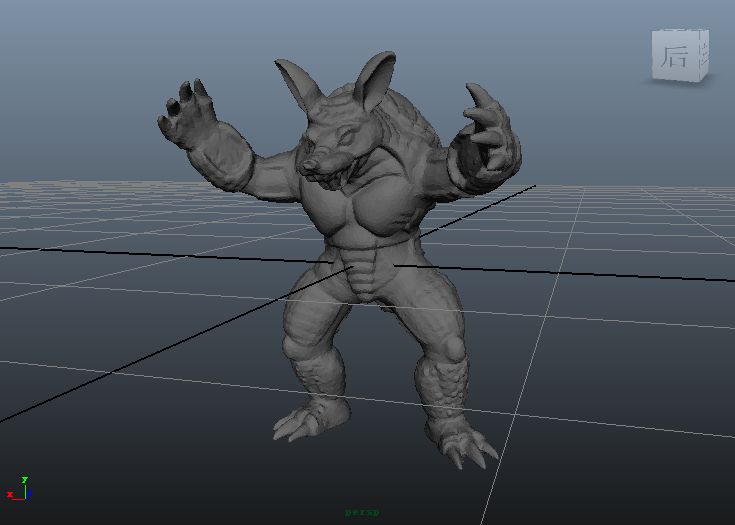
\includegraphics[width=0.3\textwidth]{1.png}}
  \subfloat[$\times$0.2 \ 3.973s]{
    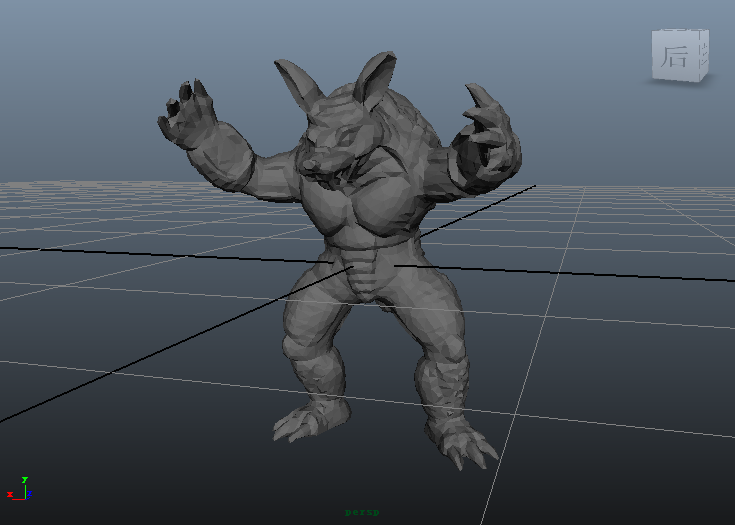
\includegraphics[width=0.3\textwidth]{2.png}}
  \subfloat[$\times$0.05 \ 4.112s]{
    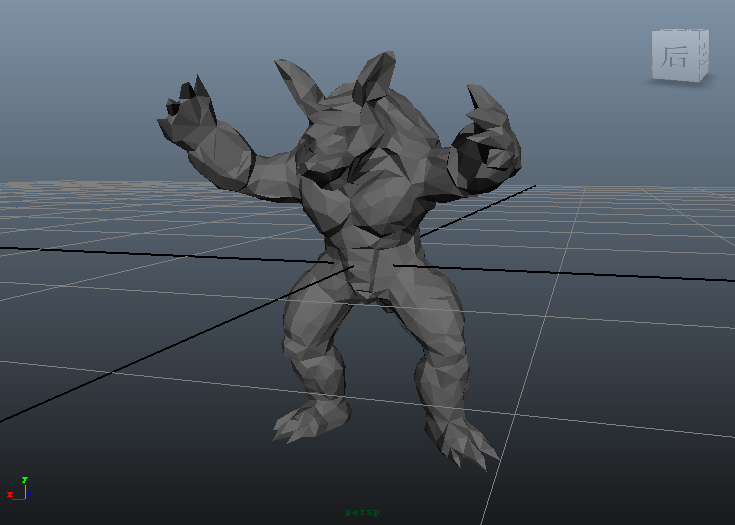
\includegraphics[width=0.3\textwidth]{3.png}}
  \caption{怪兽}
\end{figure}
\begin{figure}[H]
  \centering%
  \subfloat[$\times$1.0 \ 209227 \ faces]{
    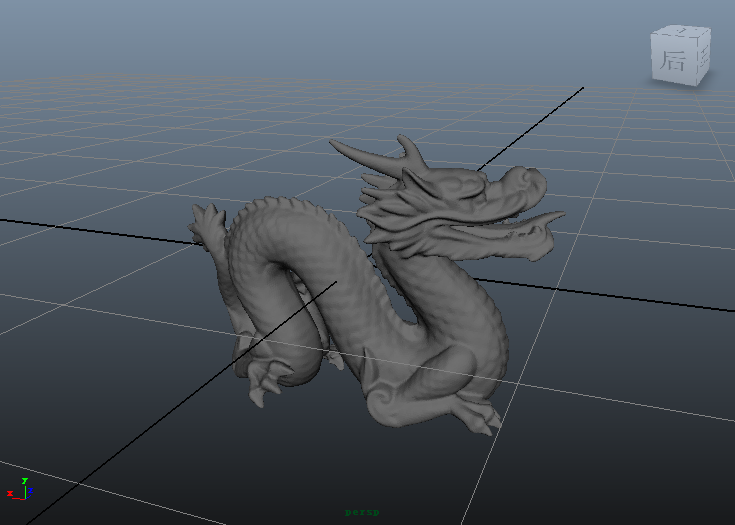
\includegraphics[width=0.3\textwidth]{4.png}}
  \subfloat[$\times$0.05 \ 107.7s]{
    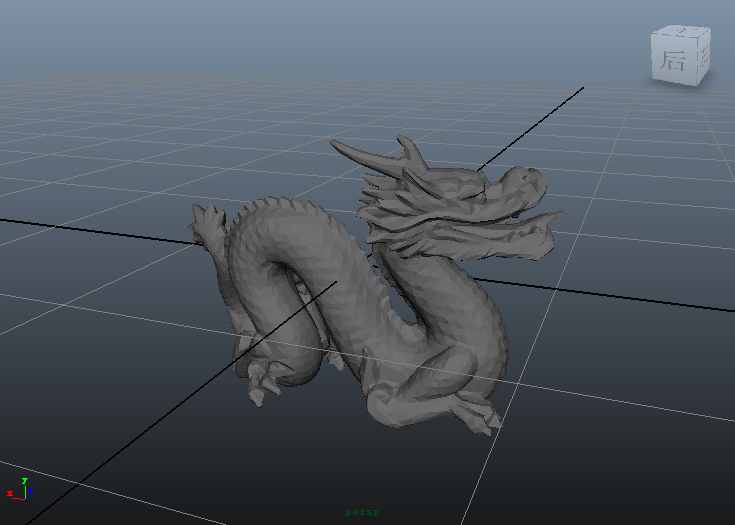
\includegraphics[width=0.3\textwidth]{5.png}}
  \subfloat[$\times$0.002 \ 107.9s]{
    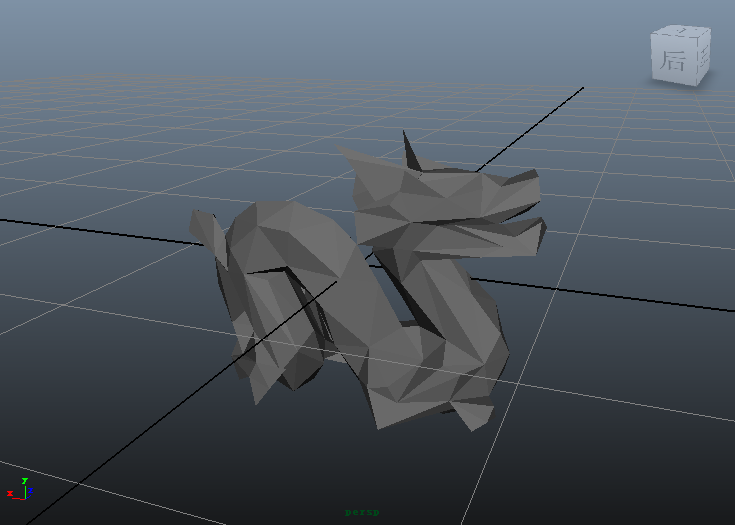
\includegraphics[width=0.3\textwidth]{6.png}}
  \caption{龙}
\end{figure}
\section{实验总结}
本次实验实现了基于二次误差度量的网格简化算法,了解了网格简化的基本思想,也实现了非边的顶点对的合并(阈值设为整个模型尺寸的0.1倍)。\par
\begin{figure}[H]
  \centering%
    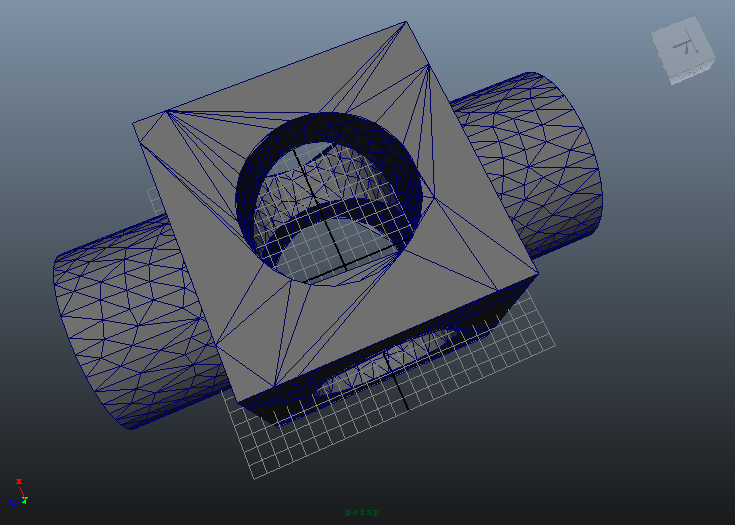
\includegraphics[width=0.5\textwidth]{7.png}
  \caption{存在的问题}
  \label{fig:cp}
\end{figure}
当然出现了一些问题,浮点误差导致的bug,堆中的边收缩和模型中的边收缩没有同步导致的bug等。除了已经解决的问题,还有一些问题没有解救,例如在比较特殊的模型中,边收缩会导致一些奇怪的现象,如图~\ref{fig:cp},在中间圆形的边缘,效果不是很好,还没有得到很好的解决。
有关网格简化,还有一些更好的方法,希望以后可以继续学习。最后感谢老师和助教的帮助。
\newpage

\addcontentsline{toc}{section}{参考文献}
\bibliography{ref/refs}
\end{document}

